\documentclass[twoside]{book}

% Packages required by doxygen
\usepackage{fixltx2e}
\usepackage{calc}
\usepackage{doxygen}
\usepackage[export]{adjustbox} % also loads graphicx
\usepackage{graphicx}
\usepackage[utf8]{inputenc}
\usepackage{makeidx}
\usepackage{multicol}
\usepackage{multirow}
\PassOptionsToPackage{warn}{textcomp}
\usepackage{textcomp}
\usepackage[nointegrals]{wasysym}
\usepackage[table]{xcolor}

% Font selection
\usepackage[T1]{fontenc}
\usepackage[scaled=.90]{helvet}
\usepackage{courier}
\usepackage{amssymb}
\usepackage{sectsty}
\renewcommand{\familydefault}{\sfdefault}
\allsectionsfont{%
  \fontseries{bc}\selectfont%
  \color{darkgray}%
}
\renewcommand{\DoxyLabelFont}{%
  \fontseries{bc}\selectfont%
  \color{darkgray}%
}
\newcommand{\+}{\discretionary{\mbox{\scriptsize$\hookleftarrow$}}{}{}}

% Page & text layout
\usepackage{geometry}
\geometry{%
  a4paper,%
  top=2.5cm,%
  bottom=2.5cm,%
  left=2.5cm,%
  right=2.5cm%
}
\tolerance=750
\hfuzz=15pt
\hbadness=750
\setlength{\emergencystretch}{15pt}
\setlength{\parindent}{0cm}
\setlength{\parskip}{3ex plus 2ex minus 2ex}
\makeatletter
\renewcommand{\paragraph}{%
  \@startsection{paragraph}{4}{0ex}{-1.0ex}{1.0ex}{%
    \normalfont\normalsize\bfseries\SS@parafont%
  }%
}
\renewcommand{\subparagraph}{%
  \@startsection{subparagraph}{5}{0ex}{-1.0ex}{1.0ex}{%
    \normalfont\normalsize\bfseries\SS@subparafont%
  }%
}
\makeatother

% Headers & footers
\usepackage{fancyhdr}
\pagestyle{fancyplain}
\fancyhead[LE]{\fancyplain{}{\bfseries\thepage}}
\fancyhead[CE]{\fancyplain{}{}}
\fancyhead[RE]{\fancyplain{}{\bfseries\leftmark}}
\fancyhead[LO]{\fancyplain{}{\bfseries\rightmark}}
\fancyhead[CO]{\fancyplain{}{}}
\fancyhead[RO]{\fancyplain{}{\bfseries\thepage}}
\fancyfoot[LE]{\fancyplain{}{}}
\fancyfoot[CE]{\fancyplain{}{}}
\fancyfoot[RE]{\fancyplain{}{\bfseries\scriptsize Generated by Doxygen }}
\fancyfoot[LO]{\fancyplain{}{\bfseries\scriptsize Generated by Doxygen }}
\fancyfoot[CO]{\fancyplain{}{}}
\fancyfoot[RO]{\fancyplain{}{}}
\renewcommand{\footrulewidth}{0.4pt}
\renewcommand{\chaptermark}[1]{%
  \markboth{#1}{}%
}
\renewcommand{\sectionmark}[1]{%
  \markright{\thesection\ #1}%
}

% Indices & bibliography
\usepackage{natbib}
\usepackage[titles]{tocloft}
\setcounter{tocdepth}{3}
\setcounter{secnumdepth}{5}
\makeindex

% Hyperlinks (required, but should be loaded last)
\usepackage{ifpdf}
\ifpdf
  \usepackage[pdftex,pagebackref=true]{hyperref}
\else
  \usepackage[ps2pdf,pagebackref=true]{hyperref}
\fi
\hypersetup{%
  colorlinks=true,%
  linkcolor=blue,%
  citecolor=blue,%
  unicode%
}

% Custom commands
\newcommand{\clearemptydoublepage}{%
  \newpage{\pagestyle{empty}\cleardoublepage}%
}

\usepackage{caption}
\captionsetup{labelsep=space,justification=centering,font={bf},singlelinecheck=off,skip=4pt,position=top}

%===== C O N T E N T S =====

\begin{document}

% Titlepage & ToC
\hypersetup{pageanchor=false,
             bookmarksnumbered=true,
             pdfencoding=unicode
            }
\pagenumbering{alph}
\begin{titlepage}
\vspace*{7cm}
\begin{center}%
{\Large Edge Detection }\\
\vspace*{1cm}
{\large Generated by Doxygen 1.8.14}\\
\end{center}
\end{titlepage}
\clearemptydoublepage
\pagenumbering{roman}
\tableofcontents
\clearemptydoublepage
\pagenumbering{arabic}
\hypersetup{pageanchor=true}

%--- Begin generated contents ---
\chapter{Namespace Index}
\section{Namespace List}
Here is a list of all documented namespaces with brief descriptions\+:\begin{DoxyCompactList}
\item\contentsline{section}{\mbox{\hyperlink{namespaceed}{ed}} \\*This namespace contains every function related to the used Canny edge detection }{\pageref{namespaceed}}{}
\item\contentsline{section}{\mbox{\hyperlink{namespacetr}{tr}} \\*This namespace contains every function related to the thresholding }{\pageref{namespacetr}}{}
\end{DoxyCompactList}

\chapter{Hierarchical Index}
\section{Class Hierarchy}
This inheritance list is sorted roughly, but not completely, alphabetically\+:\begin{DoxyCompactList}
\item \contentsline{section}{ed\+:\+:matrix$<$ T, Height, Width $>$}{\pageref{classed_1_1matrix}}{}
\item Pre\+Processing\begin{DoxyCompactList}
\item \contentsline{section}{Student\+Pre\+Processing}{\pageref{class_student_pre_processing}}{}
\end{DoxyCompactList}
\end{DoxyCompactList}

\chapter{Class Index}
\section{Class List}
Here are the classes, structs, unions and interfaces with brief descriptions\+:\begin{DoxyCompactList}
\item\contentsline{section}{\mbox{\hyperlink{classed_1_1matrix}{ed\+::matrix$<$ T, Height, Width $>$}} }{\pageref{classed_1_1matrix}}{}
\item\contentsline{section}{\mbox{\hyperlink{class_student_pre_processing}{Student\+Pre\+Processing}} }{\pageref{class_student_pre_processing}}{}
\end{DoxyCompactList}

\chapter{Namespace Documentation}
\hypertarget{namespaceed}{}\section{ed Namespace Reference}
\label{namespaceed}\index{ed@{ed}}


This namespace contains every function related to the used Canny edge detection.  


\subsection*{Classes}
\begin{DoxyCompactItemize}
\item 
class \mbox{\hyperlink{classed_1_1matrix}{matrix}}
\end{DoxyCompactItemize}
\subsection*{Functions}
\begin{DoxyCompactItemize}
\item 
{\footnotesize template$<$typename T , int Height, int Width, typename TT  = T$>$ }\\\mbox{\hyperlink{classed_1_1matrix}{matrix}}$<$ T $>$ \mbox{\hyperlink{namespaceed_aebe10857e20c7b3f680ce43f411d9492}{convolution}} (\mbox{\hyperlink{classed_1_1matrix}{matrix}}$<$ T $>$ \&image, const \mbox{\hyperlink{classed_1_1matrix}{matrix}}$<$ TT, Height, Width $>$ \&kernel)
\begin{DoxyCompactList}\small\item\em This function convolutes a matrix with another matrix. This function multiplies the first parameter matrix(image) with the second parameter matrix(kernel). \end{DoxyCompactList}\end{DoxyCompactItemize}


\subsection{Detailed Description}
This namespace contains every function related to the used Canny edge detection. 

\subsection{Function Documentation}
\mbox{\Hypertarget{namespaceed_aebe10857e20c7b3f680ce43f411d9492}\label{namespaceed_aebe10857e20c7b3f680ce43f411d9492}} 
\index{ed@{ed}!convolution@{convolution}}
\index{convolution@{convolution}!ed@{ed}}
\subsubsection{\texorpdfstring{convolution()}{convolution()}}
{\footnotesize\ttfamily template$<$typename T , int Height, int Width, typename TT  = T$>$ \\
\mbox{\hyperlink{classed_1_1matrix}{matrix}}$<$T$>$ ed\+::convolution (\begin{DoxyParamCaption}\item[{\mbox{\hyperlink{classed_1_1matrix}{matrix}}$<$ T $>$ \&}]{image,  }\item[{const \mbox{\hyperlink{classed_1_1matrix}{matrix}}$<$ TT, Height, Width $>$ \&}]{kernel }\end{DoxyParamCaption})}



This function convolutes a matrix with another matrix. This function multiplies the first parameter matrix(image) with the second parameter matrix(kernel). 


\begin{DoxyParams}{Parameters}
{\em image} & Is the matrix which is going to be convoluted by the second matrix (kernel). \\
\hline
{\em kernel} & Is the matrix which is the kernel which the image is going to be multiplied with.\\
\hline
\end{DoxyParams}
\begin{DoxyReturn}{Returns}
A new matrix as result from the convoluted picture with the kernel. 
\end{DoxyReturn}

\hypertarget{namespacetr}{}\section{tr Namespace Reference}
\label{namespacetr}\index{tr@{tr}}


This namespace contains every function related to the thresholding.  


\subsection*{Functions}
\begin{DoxyCompactItemize}
\item 
{\footnotesize template$<$class T $>$ }\\void \mbox{\hyperlink{namespacetr_a1336850c33551f00835c293b3a534c26}{basic\+\_\+threshold}} (\mbox{\hyperlink{classed_1_1matrix}{ed\+::matrix}}$<$ T $>$ \&src, const int \&threshold\+\_\+min=170, const int \&threshold\+\_\+max=2500)
\begin{DoxyCompactList}\small\item\em Thresholding for Canny edge detection This function is a static implementation of a thresholding function which means that the values that are going to be 0 if its below the threshold or 255 if above. \end{DoxyCompactList}\end{DoxyCompactItemize}


\subsection{Detailed Description}
This namespace contains every function related to the thresholding. 

\subsection{Function Documentation}
\mbox{\Hypertarget{namespacetr_a1336850c33551f00835c293b3a534c26}\label{namespacetr_a1336850c33551f00835c293b3a534c26}} 
\index{tr@{tr}!basic\+\_\+threshold@{basic\+\_\+threshold}}
\index{basic\+\_\+threshold@{basic\+\_\+threshold}!tr@{tr}}
\subsubsection{\texorpdfstring{basic\+\_\+threshold()}{basic\_threshold()}}
{\footnotesize\ttfamily template$<$class T $>$ \\
void tr\+::basic\+\_\+threshold (\begin{DoxyParamCaption}\item[{\mbox{\hyperlink{classed_1_1matrix}{ed\+::matrix}}$<$ T $>$ \&}]{src,  }\item[{const int \&}]{threshold\+\_\+min = {\ttfamily 170},  }\item[{const int \&}]{threshold\+\_\+max = {\ttfamily 2500} }\end{DoxyParamCaption})}



Thresholding for Canny edge detection This function is a static implementation of a thresholding function which means that the values that are going to be 0 if its below the threshold or 255 if above. 


\begin{DoxyParams}{Parameters}
{\em src} & The original image to apply threshold to \\
\hline
{\em threshold} & The threshold trigger to split the image \\
\hline
\end{DoxyParams}

\chapter{Class Documentation}
\hypertarget{classed_1_1matrix}{}\section{ed\+:\+:matrix$<$ T, Height, Width $>$ Class Template Reference}
\label{classed_1_1matrix}\index{ed\+::matrix$<$ T, Height, Width $>$@{ed\+::matrix$<$ T, Height, Width $>$}}


{\ttfamily \#include $<$edge\+\_\+detection.\+h$>$}

\subsection*{Public Member Functions}
\begin{DoxyCompactItemize}
\item 
constexpr \mbox{\hyperlink{classed_1_1matrix_a41874c674fa70fc0d6e6f3cce1825cfe}{matrix}} (const int height, const int width)
\item 
\mbox{\hyperlink{classed_1_1matrix_ac61570a638973eb5377cbca411ab9492}{matrix}} (const Intensity\+Image \&image)
\item 
{\footnotesize template$<$typename TT  = T$>$ }\\\mbox{\hyperlink{classed_1_1matrix_a96f0856011866bbcf92521bbf5ef9dd3}{matrix}} (const std\+::array$<$ std\+::array$<$ TT, Width $>$, Height $>$ \&\mbox{\hyperlink{classed_1_1matrix}{matrix}})
\item 
Intensity\+Image $\ast$ \mbox{\hyperlink{classed_1_1matrix_a2adb72ad2c0829cf6efc33d6984308e6}{get\+\_\+intensity\+\_\+image\+\_\+ptr}} ()
\begin{DoxyCompactList}\small\item\em This function creates and returns an new Intensity\+Image pointer. This function creates a Intensity\+Image pointer from the matrix and returns the pointer afterwards. \end{DoxyCompactList}\item 
{\footnotesize template$<$typename NT  = unsigned int$>$ }\\void \mbox{\hyperlink{classed_1_1matrix_a49e7d0658023caeafc6cf25385b74872}{equalization}} (int spread\+\_\+size)
\begin{DoxyCompactList}\small\item\em Non-\/lineair equalization. \end{DoxyCompactList}\item 
\mbox{\Hypertarget{classed_1_1matrix_a9188ac4fe9ddc17b80e9b7865f3efe12}\label{classed_1_1matrix_a9188ac4fe9ddc17b80e9b7865f3efe12}} 
{\footnotesize template$<$unsigned Min\+Value = 0, unsigned Max\+Value = 255$>$ }\\void \mbox{\hyperlink{classed_1_1matrix_a9188ac4fe9ddc17b80e9b7865f3efe12}{thresholding\+\_\+static}} ()
\begin{DoxyCompactList}\small\item\em Thresholding for Canny edge detection This function is a static implementation of a thresholding function which means that the values that are going to be Min\+Value and Max\+Value are allready known. \end{DoxyCompactList}\item 
T \& \mbox{\hyperlink{classed_1_1matrix_a958041dd0f380db0f0b60f85b736b020}{operator()}} (const int y, const int x)
\item 
T \mbox{\hyperlink{classed_1_1matrix_a6c184e083e3849cb0804915300d68cad}{operator()}} (const int y, const int x) const
\item 
T \& \mbox{\hyperlink{classed_1_1matrix_aee4710cd7dd60dc960087bc3466d2881}{operator()}} (int n)
\item 
T \mbox{\hyperlink{classed_1_1matrix_ac3928d0287a81060742db500412e530e}{operator()}} (int n) const
\end{DoxyCompactItemize}
\subsection*{Public Attributes}
\begin{DoxyCompactItemize}
\item 
\mbox{\Hypertarget{classed_1_1matrix_a57e56f840d1afa119dadee00c909b126}\label{classed_1_1matrix_a57e56f840d1afa119dadee00c909b126}} 
int {\bfseries width} = -\/1
\item 
\mbox{\Hypertarget{classed_1_1matrix_ac5c960e6811fc4f17a465e31dc216c49}\label{classed_1_1matrix_ac5c960e6811fc4f17a465e31dc216c49}} 
int {\bfseries height} = -\/1
\item 
\mbox{\Hypertarget{classed_1_1matrix_ad97cb578ebad45bf4fc7925379a3fa9f}\label{classed_1_1matrix_ad97cb578ebad45bf4fc7925379a3fa9f}} 
T $\ast$ {\bfseries m}
\end{DoxyCompactItemize}
\subsection*{Protected Member Functions}
\begin{DoxyCompactItemize}
\item 
\mbox{\Hypertarget{classed_1_1matrix_a1f388c37205e6d5443b074719cedd7d9}\label{classed_1_1matrix_a1f388c37205e6d5443b074719cedd7d9}} 
std\+::map$<$ int, unsigned int $>$ {\bfseries cdf\+\_\+map} ()
\end{DoxyCompactItemize}


\subsection{Detailed Description}
\subsubsection*{template$<$class T, int Height = 0, int Width = 0$>$\newline
class ed\+::matrix$<$ T, Height, Width $>$}

The matrix class can be used for 2D matrixes. The matrix contains some functions that are handy for working with the H\+U-\/\+Vision code structure. 

\subsection{Constructor \& Destructor Documentation}
\mbox{\Hypertarget{classed_1_1matrix_a41874c674fa70fc0d6e6f3cce1825cfe}\label{classed_1_1matrix_a41874c674fa70fc0d6e6f3cce1825cfe}} 
\index{ed\+::matrix@{ed\+::matrix}!matrix@{matrix}}
\index{matrix@{matrix}!ed\+::matrix@{ed\+::matrix}}
\subsubsection{\texorpdfstring{matrix()}{matrix()}\hspace{0.1cm}{\footnotesize\ttfamily [1/3]}}
{\footnotesize\ttfamily template$<$class T, int Height = 0, int Width = 0$>$ \\
constexpr \mbox{\hyperlink{classed_1_1matrix}{ed\+::matrix}}$<$ T, Height, Width $>$\+::\mbox{\hyperlink{classed_1_1matrix}{matrix}} (\begin{DoxyParamCaption}\item[{const int}]{height,  }\item[{const int}]{width }\end{DoxyParamCaption})\hspace{0.3cm}{\ttfamily [inline]}}

The constructor for creating an empty matrix by giving the height and width.


\begin{DoxyParams}{Parameters}
{\em height} & The height of the matrix \\
\hline
{\em width} & The width of the matrix \\
\hline
\end{DoxyParams}
\mbox{\Hypertarget{classed_1_1matrix_ac61570a638973eb5377cbca411ab9492}\label{classed_1_1matrix_ac61570a638973eb5377cbca411ab9492}} 
\index{ed\+::matrix@{ed\+::matrix}!matrix@{matrix}}
\index{matrix@{matrix}!ed\+::matrix@{ed\+::matrix}}
\subsubsection{\texorpdfstring{matrix()}{matrix()}\hspace{0.1cm}{\footnotesize\ttfamily [2/3]}}
{\footnotesize\ttfamily template$<$class T, int Height = 0, int Width = 0$>$ \\
\mbox{\hyperlink{classed_1_1matrix}{ed\+::matrix}}$<$ T, Height, Width $>$\+::\mbox{\hyperlink{classed_1_1matrix}{matrix}} (\begin{DoxyParamCaption}\item[{const Intensity\+Image \&}]{image }\end{DoxyParamCaption})\hspace{0.3cm}{\ttfamily [inline]}}

The constructor for creating a matrix from an Intensity\+Image.


\begin{DoxyParams}{Parameters}
{\em image} & An Intensity\+Image \\
\hline
\end{DoxyParams}
\mbox{\Hypertarget{classed_1_1matrix_a96f0856011866bbcf92521bbf5ef9dd3}\label{classed_1_1matrix_a96f0856011866bbcf92521bbf5ef9dd3}} 
\index{ed\+::matrix@{ed\+::matrix}!matrix@{matrix}}
\index{matrix@{matrix}!ed\+::matrix@{ed\+::matrix}}
\subsubsection{\texorpdfstring{matrix()}{matrix()}\hspace{0.1cm}{\footnotesize\ttfamily [3/3]}}
{\footnotesize\ttfamily template$<$class T, int Height = 0, int Width = 0$>$ \\
template$<$typename TT  = T$>$ \\
\mbox{\hyperlink{classed_1_1matrix}{ed\+::matrix}}$<$ T, Height, Width $>$\+::\mbox{\hyperlink{classed_1_1matrix}{matrix}} (\begin{DoxyParamCaption}\item[{const std\+::array$<$ std\+::array$<$ TT, Width $>$, Height $>$ \&}]{matrix }\end{DoxyParamCaption})\hspace{0.3cm}{\ttfamily [inline]}}

The constructor for creating a copy of another matrix.


\begin{DoxyParams}{Parameters}
{\em matrix} & The matrix which going to be copied. \\
\hline
\end{DoxyParams}


\subsection{Member Function Documentation}
\mbox{\Hypertarget{classed_1_1matrix_a49e7d0658023caeafc6cf25385b74872}\label{classed_1_1matrix_a49e7d0658023caeafc6cf25385b74872}} 
\index{ed\+::matrix@{ed\+::matrix}!equalization@{equalization}}
\index{equalization@{equalization}!ed\+::matrix@{ed\+::matrix}}
\subsubsection{\texorpdfstring{equalization()}{equalization()}}
{\footnotesize\ttfamily template$<$class T, int Height = 0, int Width = 0$>$ \\
template$<$typename NT  = unsigned int$>$ \\
void \mbox{\hyperlink{classed_1_1matrix}{ed\+::matrix}}$<$ T, Height, Width $>$\+::equalization (\begin{DoxyParamCaption}\item[{int}]{spread\+\_\+size }\end{DoxyParamCaption})\hspace{0.3cm}{\ttfamily [inline]}}



Non-\/lineair equalization. 

This equalization function makes use of the non-\/lineair way of equalization with the result of distributing a pixel value according to the frequency of the original pixel value. This function scales the values $<$=0 to 0 with as maximum the spread\+\_\+size value.


\begin{DoxyParams}{Parameters}
{\em spread\+\_\+size} & The equialized values are in a range from 0 and spread\+\_\+size. \\
\hline
\end{DoxyParams}
\mbox{\Hypertarget{classed_1_1matrix_a2adb72ad2c0829cf6efc33d6984308e6}\label{classed_1_1matrix_a2adb72ad2c0829cf6efc33d6984308e6}} 
\index{ed\+::matrix@{ed\+::matrix}!get\+\_\+intensity\+\_\+image\+\_\+ptr@{get\+\_\+intensity\+\_\+image\+\_\+ptr}}
\index{get\+\_\+intensity\+\_\+image\+\_\+ptr@{get\+\_\+intensity\+\_\+image\+\_\+ptr}!ed\+::matrix@{ed\+::matrix}}
\subsubsection{\texorpdfstring{get\+\_\+intensity\+\_\+image\+\_\+ptr()}{get\_intensity\_image\_ptr()}}
{\footnotesize\ttfamily template$<$class T, int Height = 0, int Width = 0$>$ \\
Intensity\+Image$\ast$ \mbox{\hyperlink{classed_1_1matrix}{ed\+::matrix}}$<$ T, Height, Width $>$\+::get\+\_\+intensity\+\_\+image\+\_\+ptr (\begin{DoxyParamCaption}{ }\end{DoxyParamCaption})\hspace{0.3cm}{\ttfamily [inline]}}



This function creates and returns an new Intensity\+Image pointer. This function creates a Intensity\+Image pointer from the matrix and returns the pointer afterwards. 

\begin{DoxyReturn}{Returns}
The Intensity\+Image pointer. 
\end{DoxyReturn}
\mbox{\Hypertarget{classed_1_1matrix_a958041dd0f380db0f0b60f85b736b020}\label{classed_1_1matrix_a958041dd0f380db0f0b60f85b736b020}} 
\index{ed\+::matrix@{ed\+::matrix}!operator()@{operator()}}
\index{operator()@{operator()}!ed\+::matrix@{ed\+::matrix}}
\subsubsection{\texorpdfstring{operator()()}{operator()()}\hspace{0.1cm}{\footnotesize\ttfamily [1/4]}}
{\footnotesize\ttfamily template$<$class T, int Height = 0, int Width = 0$>$ \\
T\& \mbox{\hyperlink{classed_1_1matrix}{ed\+::matrix}}$<$ T, Height, Width $>$\+::operator() (\begin{DoxyParamCaption}\item[{const int}]{y,  }\item[{const int}]{x }\end{DoxyParamCaption})\hspace{0.3cm}{\ttfamily [inline]}}

Operator for using the 1D array as an 2D array.


\begin{DoxyParams}{Parameters}
{\em y} & The height value (y). \\
\hline
{\em x} & The width value (x).\\
\hline
\end{DoxyParams}
\begin{DoxyReturn}{Returns}
The reference to the value of (y, x). 
\end{DoxyReturn}
\mbox{\Hypertarget{classed_1_1matrix_a6c184e083e3849cb0804915300d68cad}\label{classed_1_1matrix_a6c184e083e3849cb0804915300d68cad}} 
\index{ed\+::matrix@{ed\+::matrix}!operator()@{operator()}}
\index{operator()@{operator()}!ed\+::matrix@{ed\+::matrix}}
\subsubsection{\texorpdfstring{operator()()}{operator()()}\hspace{0.1cm}{\footnotesize\ttfamily [2/4]}}
{\footnotesize\ttfamily template$<$class T, int Height = 0, int Width = 0$>$ \\
T \mbox{\hyperlink{classed_1_1matrix}{ed\+::matrix}}$<$ T, Height, Width $>$\+::operator() (\begin{DoxyParamCaption}\item[{const int}]{y,  }\item[{const int}]{x }\end{DoxyParamCaption}) const\hspace{0.3cm}{\ttfamily [inline]}}

Operator for using the 1D array as an 2D array.


\begin{DoxyParams}{Parameters}
{\em y} & The height value (y). \\
\hline
{\em x} & The width value (x).\\
\hline
\end{DoxyParams}
\begin{DoxyReturn}{Returns}
The value of (y, x). 
\end{DoxyReturn}
\mbox{\Hypertarget{classed_1_1matrix_aee4710cd7dd60dc960087bc3466d2881}\label{classed_1_1matrix_aee4710cd7dd60dc960087bc3466d2881}} 
\index{ed\+::matrix@{ed\+::matrix}!operator()@{operator()}}
\index{operator()@{operator()}!ed\+::matrix@{ed\+::matrix}}
\subsubsection{\texorpdfstring{operator()()}{operator()()}\hspace{0.1cm}{\footnotesize\ttfamily [3/4]}}
{\footnotesize\ttfamily template$<$class T, int Height = 0, int Width = 0$>$ \\
T\& \mbox{\hyperlink{classed_1_1matrix}{ed\+::matrix}}$<$ T, Height, Width $>$\+::operator() (\begin{DoxyParamCaption}\item[{int}]{n }\end{DoxyParamCaption})\hspace{0.3cm}{\ttfamily [inline]}}

Operator for using the 1D array with a direct index.


\begin{DoxyParams}{Parameters}
{\em n} & The index of the array.\\
\hline
\end{DoxyParams}
\begin{DoxyReturn}{Returns}
The reference to the value of (n). 
\end{DoxyReturn}
\mbox{\Hypertarget{classed_1_1matrix_ac3928d0287a81060742db500412e530e}\label{classed_1_1matrix_ac3928d0287a81060742db500412e530e}} 
\index{ed\+::matrix@{ed\+::matrix}!operator()@{operator()}}
\index{operator()@{operator()}!ed\+::matrix@{ed\+::matrix}}
\subsubsection{\texorpdfstring{operator()()}{operator()()}\hspace{0.1cm}{\footnotesize\ttfamily [4/4]}}
{\footnotesize\ttfamily template$<$class T, int Height = 0, int Width = 0$>$ \\
T \mbox{\hyperlink{classed_1_1matrix}{ed\+::matrix}}$<$ T, Height, Width $>$\+::operator() (\begin{DoxyParamCaption}\item[{int}]{n }\end{DoxyParamCaption}) const\hspace{0.3cm}{\ttfamily [inline]}}

Operator for using the 1D array with a direct index.


\begin{DoxyParams}{Parameters}
{\em n} & The index of the array.\\
\hline
\end{DoxyParams}
\begin{DoxyReturn}{Returns}
The value of (n). 
\end{DoxyReturn}


The documentation for this class was generated from the following file\+:\begin{DoxyCompactItemize}
\item 
edge\+\_\+detection.\+h\end{DoxyCompactItemize}

\hypertarget{class_student_pre_processing}{}\section{Student\+Pre\+Processing Class Reference}
\label{class_student_pre_processing}\index{Student\+Pre\+Processing@{Student\+Pre\+Processing}}
Inheritance diagram for Student\+Pre\+Processing\+:\begin{figure}[H]
\begin{center}
\leavevmode
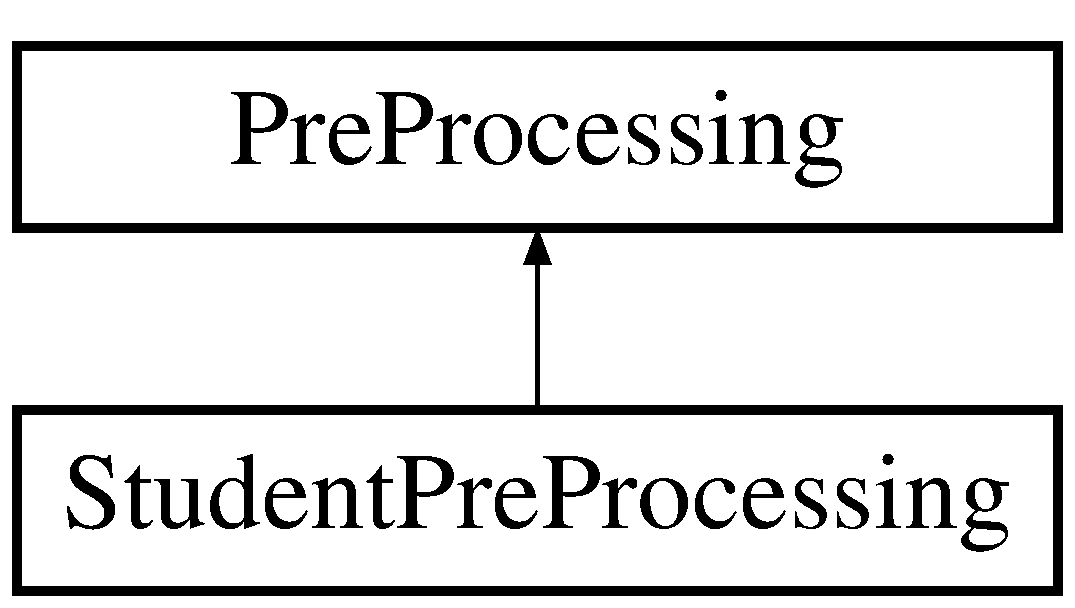
\includegraphics[height=2.000000cm]{class_student_pre_processing}
\end{center}
\end{figure}
\subsection*{Public Member Functions}
\begin{DoxyCompactItemize}
\item 
\mbox{\Hypertarget{class_student_pre_processing_ab41148b8a4701cda08e67d2ad4a61747}\label{class_student_pre_processing_ab41148b8a4701cda08e67d2ad4a61747}} 
Intensity\+Image $\ast$ \mbox{\hyperlink{class_student_pre_processing_ab41148b8a4701cda08e67d2ad4a61747}{step\+Edge\+Detection}} (const Intensity\+Image \&image) const
\begin{DoxyCompactList}\small\item\em biertje \end{DoxyCompactList}\item 
Intensity\+Image $\ast$ \mbox{\hyperlink{class_student_pre_processing_a7e16ec24f25b582dfd9d2de63ce664e6}{step\+Thresholding}} (const Intensity\+Image \&image) const
\begin{DoxyCompactList}\small\item\em We don\textquotesingle{}t use this function. \end{DoxyCompactList}\end{DoxyCompactItemize}


\subsection{Member Function Documentation}
\mbox{\Hypertarget{class_student_pre_processing_a7e16ec24f25b582dfd9d2de63ce664e6}\label{class_student_pre_processing_a7e16ec24f25b582dfd9d2de63ce664e6}} 
\index{Student\+Pre\+Processing@{Student\+Pre\+Processing}!step\+Thresholding@{step\+Thresholding}}
\index{step\+Thresholding@{step\+Thresholding}!Student\+Pre\+Processing@{Student\+Pre\+Processing}}
\subsubsection{\texorpdfstring{step\+Thresholding()}{stepThresholding()}}
{\footnotesize\ttfamily Intensity\+Image$\ast$ Student\+Pre\+Processing\+::step\+Thresholding (\begin{DoxyParamCaption}\item[{const Intensity\+Image \&}]{image }\end{DoxyParamCaption}) const}



We don\textquotesingle{}t use this function. 

We don\textquotesingle{}t use this function becouse we do the thresholding in the edge detection function. Read the documentation for more information.

\begin{DoxyReturn}{Returns}
This function returns an img\+\_\+ptr copied from the step\+Edge\+Detection function 
\end{DoxyReturn}


The documentation for this class was generated from the following file\+:\begin{DoxyCompactItemize}
\item 
Student\+Pre\+Processing.\+h\end{DoxyCompactItemize}

%--- End generated contents ---

% Index
\backmatter
\newpage
\phantomsection
\clearemptydoublepage
\addcontentsline{toc}{chapter}{Index}
\printindex

\end{document}
